%Copyright 2014 Jean-Philippe Eisenbarth
%This program is free software: you can 
%redistribute it and/or modify it under the terms of the GNU General Public 
%License as published by the Free Software Foundation, either version 3 of the 
%License, or (at your option) any later version.
%This program is distributed in the hope that it will be useful,but WITHOUT ANY 
%WARRANTY; without even the implied warranty of MERCHANTABILITY or FITNESS FOR A 
%PARTICULAR PURPOSE. See the GNU General Public License for more details.
%You should have received a copy of the GNU General Public License along with 
%this program.  If not, see <http://www.gnu.org/licenses/>.

%Based on the code of Yiannis Lazarides
%http://tex.stackexchange.com/questions/42602/software-requirements-specification-with-latex
%http://tex.stackexchange.com/users/963/yiannis-lazarides
%Also based on the template of Karl E. Wiegers
%http://www.se.rit.edu/~emad/teaching/slides/srs_template_sep14.pdf
%http://karlwiegers.com
\documentclass{scrreprt}
\usepackage{placeins}
\usepackage{listings}
\usepackage{underscore}
%\usepackage[bookmarks=true]{hyperref}
\usepackage{graphicx}
\usepackage{hyperref}
\usepackage[utf8]{inputenc}
\usepackage[english]{babel}
\usepackage{xargs}
\usepackage[pdftex,dvipsnames]{xcolor}
\usepackage[colorinlistoftodos,prependcaption,textsize=tiny]{todonotes}
\usepackage{etoolbox}
%\usepackage{hyperref}
%\usepackage{titlesec}
\usepackage{amsthm}
\usepackage{nameref}
\usepackage{zref-titleref}
\usepackage{float}
\usepackage{adjustbox}
\usepackage{graphicx}
\usepackage[normalem]{ulem}
\usepackage{tabularx}
\useunder{\uline}{\ul}{}

%\usepackage{chngcntr}
%\usepackage{thmtools}

%\makeatletter
%\patchcmd{\chapter}{\if@openright\cleardoublepage\else\clearpage\fi}{}{}{}
%\makeatother

%\makeatletter
%\newcommand{\customlabel}[2]{%
%	\protected@write \@auxout {}{\string \newlabel {#1}{{#2}{}}}}
%\makeatother


%\newcounter{funcreq}
%\titleclass{\funcreq}{straight}[\part]
%\titleformat{\funcreq}[hang]
%{\normalfont\bfseries}{\thefuncreq}{1em}{}
%\titlespacing*{\funcreq}{0pt}{3.5ex plus 1ex minus .2ex}{2.3 ex plus .2ex}
%\renewcommand{\thefuncreq}{FR\arabic{funcreq}}
%\counterwithin{section}{funcreq}
%

%\newtheoremstyle{mytheoremstyle} % name
%{\topsep}                    % Space above
%{\topsep}                    % Space below
%{\itshape}                   % Body font
%{}                           % Indent amount
%{\scshape}                   % Theorem head font
%{}                          % Punctuation after theorem head
%{0em}                       % Space after theorem head
%{}  % Theorem head spec (can be left empty, meaning ‘normal’)
%
%\theoremstyle{mytheoremstyle}


%\newcounter{funcreq}
%\makeatletter
%\newenvironment{funcreq}[1]
%{\refstepcounter{funcreq}%
%	\protected@edef\@currentlabelname{#1}% addition here
%	\vspace{0.5cm}\noindent
%	{\large\bfseries{FR\thefuncreq\par}
%	}
%}
%\makeatother

\usepackage[parfill]{parskip}

\newcounter{funcreq}
\makeatletter
\newenvironment{funcreq}
{\refstepcounter{funcreq}{}%
	
	\protected@edef\@currentlabelname
	everypar={{\setbox0=\lastbox}\thefuncreq.\hspace{4pt}\everypar={}}
	\noindent
	{
		\bfseries{FR\thefuncreq}\par\noindent
	}
	\noindent
}
{
	\par\noindent
}
\makeatother

%\newcommand*{\currentname}{\zref@getcurrent{subsection}}
\let\Subsectionmark\subsectionmark
\def\subsectionmark#1{\def\Subsectionname{#1}\Subsectionmark{#1}}

\newtheoremstyle{funreq}
{0}       % ABOVESPACE
{0}       % BELOWSPACE
{\upshape}  % BODYFONT
{0pt}       % INDENT (empty value is the same as 0pt)
{}          % HEADFONT
{}         % HEADPUNCT
{0pt}         % HEADSPACE
% CUSTOM-HEAD-SPEC follows
{\bfseries ID: FR\thmnumber{#2}\\}

\theoremstyle{funreq}
\newtheorem{funreq}{}


\def\sectionautorefname{funcreq}
\newcommand{\secref}[1]{FR\autoref{#1}}

%{%\par\noindent
%	
%	\refstepcounter{funcreq}
%	\protected@edef\@currentlabelname{#1}
%	\textbf{FR\thefuncreq}\ignorespaces}
%{\par\ignorespacesafterend}}


%\newcommand*{\fancyreffuncreqprefix}{req}

\newcommand*{\reqref}[1]{\hyperref[#1]{FR\ref*{#1}}}
\newcommand{\specialcell}[2][c]{%
	\begin{tabularx}[#1]{@{}X@{}}#2\end{tabularx}}

%\newtheorem{funcreq}{FR}


\hypersetup{
    %bookmarks=false,    % show bookmarks bar?
    pdftitle={Software Requirement Specification},    % title
    pdfauthor={Jean-Philippe Eisenbarth},                     % author
    pdfsubject={TeX and LaTeX},                        % subject of the document
    pdfkeywords={TeX, LaTeX, graphics, images}, % list of keywords
    colorlinks=true,       % false: boxed links; true: colored links
    linkcolor=blue,       % color of internal links
    citecolor=black,       % color of links to bibliography
    filecolor=black,        % color of file links
    urlcolor=purple,        % color of external links
    linktoc=page            % only page is linked
}
\def\myversion{1.0 }
\date{}
%\title
\usepackage{hyperref}

\newcommandx{\unsure}[2][1=]{\todo[linecolor=red,backgroundcolor=red!25,bordercolor=red,#1]{#2}}
\newcommandx{\change}[2][1=]{\todo[linecolor=blue,backgroundcolor=blue!25,bordercolor=blue,#1]{#2}}
\newcommandx{\info}[2][1=]{\todo[linecolor=OliveGreen,backgroundcolor=OliveGreen!25,bordercolor=OliveGreen,#1]{#2}}
\newcommandx{\improvement}[2][1=]{\todo[linecolor=YellowOrange,backgroundcolor=YellowOrange!35,bordercolor=YellowOrange,#1]{#2}}
\newcommandx{\thiswillnotshow}[2][1=]{\todo[disable,#1]{#2}}


\begin{document}

\begin{flushright}
    \rule{16cm}{5pt}\vskip1cm
    \begin{bfseries}
        \Huge{SOFTWARE REQUIREMENTS\\ SPECIFICATION}\\
        \vspace{1.9cm}
        for\\
        \vspace{1.9cm}
        Whole Knockoffs Grocery Store\\
        %\vspace{1.9cm}
        %\LARGE{Version \myversion approved}\\
        %\vspace{1.9cm}
        %Prepared by $<$author$>$\\
        %\vspace{1.9cm}
        %$<$Organization$>$\\
        \vspace{1.9cm}
        \today\\
    \end{bfseries}
\end{flushright}

\tableofcontents


%\chapter*{Revision History}
%
%\begin{center}
%    \begin{tabular}{|c|c|c|c|}
%        \hline
%	    Name & Date & Reason For Changes & Version\\
%        \hline
%	    21 & 22 & 23 & 24\\
%        \hline
%	    31 & 32 & 33 & 34\\
%        \hline
%    \end{tabular}
%\end{center}

\chapter{Introduction}

\section{Purpose}
This document provides detailed requirements about the product our team is creating for the customer.  This document is intended for the customers and the software team designing as a reference on the desired behaviors and requirements of the program.

\section{Scope}
The Whole Knockoff Grocery Store (WKGS) program is intended to be a system to allow the Whole Knockoff grocery store to manage employees, track inventory, sell groceries online (using both delivery and in-store pickup), and give discounts to loyal shoppers.  The WKGS website will allow customers to quickly see what is available to purchase at the grocery store using a storefront.  The customer can select items that they wish to purchase for delivery or in-store pickup.  After adding groceries to their virtual shopping cart, the customer can select if they would like the groceries delivered or available for in-store pickup.  The customer can then purchase these groceries through the online portal.  The website will also act as an employee hub where employees can be assigned work schedules and hours worked can be tracked.  The system should also handle the inventory management for the entire store.  The inventory should be able to communicate with the store's point of sale systems and website so that correct inventory is maintained when items are purchased.  This will allow the store owners to know what items are in-stock and which items might need to be re-ordered.

\section{Definitions, acronyms, and abbreviations}
\textit{WKGS}: Whole Knockoff Grocery Store\\
\textit{POS}: Point of Sale system - Cash registers that are used to scan and sell groceries in-store\\


\section{References}\unsure{Do we need this?}
$<$ Placeholder $>$

\section{Overview}
In section 2, the product will be given an overall description.  Section 3 will describe in detail each of the features and their corresponding requirements.   
%$<$ Placeholder $>$

{\let\clearpage\relax 
\chapter{Overall Description}}

\section{Product Perspective}
\info[inline]{This subsection of the SRS should put the product into perspective with other related products. If the product is independent and totally self-contained, it should be so stated here. If the SRS defines a product that is a component of a larger system, as frequently occurs, then this subsection should relate the requirements of that larger system to functionality of the software and should identify interfaces between that system and the software.A block diagram showing the major components of the larger system, interconnections, and external inter-faces can be helpful.  This  subsection  should  also  describe  how  the  software  operates  inside  various  constraints.  For  example,these constraints could include\bigskip
	\indent a)System interfaces;\\
	\indent b)User interfaces;\\
	\indent c)Hardware interfaces;\\
	\indent d)Software interfaces;\\
	\indent e)Communications interfaces;\\
	\indent f)Memory;\\
	\indent g)Operations;\\
	\indent h)Site adaptation requirements.}
$<$ Placeholder $>$

\section{Product Functions}
\info[inline]{This subsection of the SRS should provide a summary of the major functions that the software will perform.For example, an SRS for an accounting program may use this part to address customer account maintenance,customer statement, and invoice preparation without mentioning the vast amount of detail that each of those functions requires.  Sometimes the function summary that is necessary for this part can be taken directly from the section of the higher-level specification (if one exists) that allocates particular functions to the software product. Note that for the sake of clarity\\\bigskip
	a)The  functions  should  be  organized  in  a  way  that  makes  the  list  of  functions  understandable  to  the customer or to anyone else reading the document for the first time.\\\bigskip 
	b)Textual  or  graphical  methods  can  be  used  to  show  the  different  functions  and  their  relationships.Such a diagram is not intended to show a design of a product, but simply shows the logical relation-ships among variables.}
$<$ Placeholder $>$

\section{User Classes and Characteristics}
\info[inline]{This subsection of the SRS should describe those general characteristics of the intended users of the product including  educational  level,  experience,  and  technical  expertise.  It  should  not  be  used  to  state  specific requirements, but rather should provide the reasons why certain specific requirements are later specified in Section 3 of the SRS.}
$<$ Placeholder $>$

\section{Constraints}
\info[inline]{This subsection of the SRS should provide a general description of any other items that will limit the developer’s options. These include\\\bigskip
a)Regulatory policies;\\
b)Hardware limitations (e.g., signal timing requirements);\\
c)Interfaces to other applications;\\
d)Parallel operation;\\
e)Audit functions;\\
f)Control functions;\\
g)Higher-order language requirements;\\
h)Signal handshake protocols (e.g., XON-XOFF, ACK-NACK);\\
i)Reliability requirements;\\
j)Criticality of the application;\\
k)Safety and security considerations.\\}
$<$ Placeholder $>$

\section{Assumptions and Dependencies}
\info[inline]{This  subsection  of  the  SRS  should  list  each  of  the  factors  that  affect  the  requirements  stated  in  the  SRS.These factors are not design constraints on the software but are, rather, any changes to them that can affect the requirements in the SRS. For example, an assumption may be that a specific operating system will be available on the hardware designated for the software product. If, in fact, the operating system is not avail-able, the SRS would then have to change accordingly. }
$<$ Placeholder $>$



{\let\clearpage\relax 
\chapter{Specific requirements}}

\section{External Interface Requirements}

\subsection{User Interfaces}
$<$ Placeholder $>$

\subsection{Hardware Interfaces}
$<$ Placeholder $>$

\subsection{Software Interfaces}
$<$ Placeholder $>$

\subsection{Communications Interfaces}
$<$ Placeholder $>$

\section{System Features}

%----------------------------


\subsection{Online checkout}
	%\chapter*{Revision History}
	%
	%\begin{center}
	%    \begin{tabular}{|c|c|c|c|}
	%        \hline
	%	    Name & Date & Reason For Changes & Version\\
	%        \hline
	%	    21 & 22 & 23 & 24\\
	%        \hline
	%	    31 & 32 & 33 & 34\\
	%        \hline
	%    \end{tabular}
	%\end{center}

	%----------------------------
	
	
	\subsection{Online checkout}
	
	
	
	\improvement[inline]{\newline This section is incomplete}
	\subsubsection{Introduction/Purpose of feature}
	The checkout feature allows users to pay for their item(s) currently in the Cart list to complete their order. Depending on type of users, the feature should preload required user’s information for the checkout process including: home address for delivery, billing address, and payment method. Furthermore, the users can specify payment and delivery options on the checkout page. 
	
	\subsubsection{Stimulus/Response sequence}
	Existing users/members:
	When the “Checkout” option is clicked, the system will direct the user to the checkout page. On the checkout page, certain user information should be preloaded to help ease the checkout process. The user will have the option to use saved payment information or a different payment method. In addition, the user can select different delivery options including: in-store pickup or home delivery. If a user chooses home delivery, the system will use the user's saved home address. If the user chooses in-store pickup by car, the system will request car model information. The user will need to click “Complete Order” to process the order.
	Guest users: 
	When the “Checkout” option is clicked, the system will direct the user to the checkout page. On the checkout page, the user would need to fill in all the required information needed for the checkout process. The user must select the payment method; the system will ask for billing address and payment information. In addition, the user can select different delivery options including: in-store pickup or home delivery. If a user chooses home delivery, the system will request a home address. If the user chooses in-store pickup by car, the system will request car model information. The user will need to click “Complete Order” to process the order.
	
	
	\subsubsection{Associated functional requirements}
	
	%\paragraph[]{\normalfont \Subsectionname ~functional requirement \arabic{subsubsection}.\arabic{paragraph}}
	%\paragraph[]{\normalfont A checkout page must be available for the users to fill in the required personal information to complete the order.}
	%\paragraph[]{\normalfont A user must be logged in as an existing user/member or guest.}
	
	\paragraph[]{Functional requirement \arabic{subsubsection}.\arabic{paragraph}}
	\begin{funreq}
		\label{online_checkout}
		TITLE: Online checkout - Allow everyone to checkout online\\
		DESC: The checkout feature should allow all users to pay for their item(s) currently in the Cart list to complete their order. Depending on type of users, the feature should preload and/or request required user’s information for the checkout process including home address for delivery, billing address, and payment method. Furthermore, the users can specify payment and delivery options on the checkout page.\\
		RAT: In order for all users to pay for their online order.\\
		DEP: None\\
		
		\clearpage
		\begin{table}[htb]
			\begin{flushleft}\bfseries{ID and Name: FR\thefunreq ~\hspace{.6cm}Create a User new account}\end{flushleft}
			%\begin{adjustbox}{width=\textwidth}
			\begin{tabularx}{\columnwidth}{|X|X|X|X|}
				\hline
				Created By    & Thoai Mai & Date Created    & 03/15/2020 \\ \hline
				Primary Actor & User        & Secondary Actor & Website \\ \hline
			\end{tabularx}
			%\end{adjustbox}
		%\end{table}
		
		%\begin{table}[h!]
			\resizebox{\textwidth}{!}{%
				\begin{tabularx}{\columnwidth}{|l|X|}
					\hline
					Description: &
					
					The checkout feature should let guest user complete online order with the required information, including payment and home delivery/in-store pickup options             \\ \hline
					Trigger:         & Guest user clicks on option “checkout”                    \\ \hline
					Preconditions    & None                                       \\ \hline
					Postconditions   & Guest user successfully complete checkout for online orders, Payment received\\ \hline
					Normal Flow &
					\bfseries{Allow everyone to checkout online – Guest User}\normalfont\newline 
					Guest user selects checkout option
					
					Website checks for type of user \textit{Note: prompt for account login? Direct for different req path?}
					
					Website established guest user
					
					Website validates accurate pricing with additional taxes for total price
					
					Website requests guest user the following information: name, payment information, billing address, option for home deliver or in-store pickup
					
					Guest user select “Place Order” option
					
					Website uses third party checkout system to validate payment transaction
					
					If payment is successfully validated and received, website acknowledges “Order Place” message\\ \hline
					
					Alternative Flow & None                                       \\ \hline
					Exceptions       & Payment did not successfully validate
					
					Guest user did not fill in the required information
					\\ \hline
					Priority & High                                       \\ \hline
				\end{tabularx}%
			}
		\end{table}
		\clearpage
		\begin{table}[htb!]
			%\begin{adjustbox}{width=\textwidth}
			\begin{tabularx}{\columnwidth}{|X|X|X|X|}
				\hline
				Created By    & Thoai Mai & Date Created    & 03/15/2020 \\ \hline
				Primary Actor & Member User        & Secondary Actor & Website \\ \hline
			\end{tabularx}
			%\end{adjustbox}
		%\end{table}
		
		%\begin{table}[h!]
			\resizebox{\textwidth}{!}{%
				\begin{tabularx}{\columnwidth}{|l|X|}
					\hline
					Description: &
					
					The checkout feature should let member user complete online order with the required information, including payment and home delivery/in-store pickup options
					\\ \hline
					Trigger:         & Member user clicks on option “checkout”                    \\ \hline
					Preconditions    & Logged in as a member                                       \\ \hline
					Postconditions   & Member user successfully complete checkout for online orders, Payment received\\ \hline
					Normal Flow &
					\bfseries{Allow everyone to checkout online – Member User}\normalfont\newline 
					
					Member user selects checkout option
					
					Website checks for type of user
					
					Website established member user
					
					Website preloads member information: name and address
					
					Website validates accurate pricing with additional taxes for total price
					
					Website requests member user the following information: payment information, billing address, option for home deliver or in-store pickup \textit{Note: should website keep payment information for member}s?
					
					Guest user select “Place Order” option
					
					Website uses third party checkout system to validate payment transaction
					
					If payment is successfully validated and received, website acknowledges “Order Place” message\\ \hline
					
					Alternative Flow & None                                       \\ \hline
					Exceptions       & Payment did not successfully validate \\ \hline
					Priority & High                                       \\ \hline
				\end{tabularx}%
			}
		\end{table}
	\end{funreq}

	\subsection{Account Management System}
\improvement[inline]{\newline This section is incomplete}
\subsubsection{Introduction/Purpose of feature}
This feature allows users to create and edit settings for grocery store accounts.  New users will use this feature to populate basic account information while setting up their account such as username and password.  In addition, this feature allows existing users a convenient way to edit their password, change shipping addresses, manage stored payment information, and change other stored personal details.  From the user management profile, users will also be able to see past purchases and orders.

\subsubsection{Stimulus/Response sequence}
\indent New users: When the “sign up” button is pressed, the system will direct the user to select a username and password to create their account.  After the user fills appropriate values into these fields, the user will be able to sign in using the credentials selected.
Existing users: When the “log in” button is pressed, the system will direct the user to enter their credentials to sign into the system.  
Logged-in users: When a user is logged-in and presses the “my account” button, the user will be brought to a page where they can edit their personal details

\subsubsection{Associated functional requirements}
\paragraph[]{Functional requirement \arabic{subsubsection}.\arabic{paragraph}}

\begin{funreq}
	
	\label{account_create}
	TITLE: Create a new User account\\
	DESC: A user should be able to register through the website. The user must provide user-name, password and e-mail address. \\
	RAT: In order for a user to register an account\\
	DEP: None\\
	
	\bfseries{ID and Name: FR\thefunreq ~\hspace{.6cm}Create a User new account}
	\begin{table}[h!]
		%\begin{adjustbox}{width=\textwidth}
		\begin{tabularx}{\columnwidth}{|X|X|X|X|}
			\hline
			Created By    & Emmanuel .W & Date Created    & 03/13/13 \\ \hline
			Primary Actor & User        & Secondary Actor & Website \\ \hline
		\end{tabularx}
		%\end{adjustbox}
		%\end{table}
		
		%\begin{table}[h!]
		\resizebox{\textwidth}{!}{%
			\begin{tabularx}{\columnwidth}{|l|X|}
				\hline
				Description: &
				A user should be able to register through the website. The user must provide a name, user-name, password and e-mail address. \\ \hline
				Trigger:         & User Clicks on register                    \\ \hline
				Preconditions    & None                                       \\ \hline
				Postconditions   & Account is created, User is Logged in      \\ \hline
				Normal Flow &
				\bfseries{Create a User new account}\normalfont\newline 
				User Clicks on Register Enters name, user-name, password and e-mail address.\newline
				Website confirms it is a unique entry and save the new user details\newline
				Website Informs User of successful creation\newline
				Website Logs user in \\ \hline
				Alternative Flow & None                                       \\ \hline
				Exceptions       & Email Address already exists in the system \\ \hline
				Priority         & High                                       \\ \hline
			\end{tabularx}%
		}
	\end{table}
\end{funreq}

\paragraph[]{Functional requirement \arabic{subsubsection}.\arabic{paragraph}}
\begin{funreq}
	\label{account_createstaff}
	TITLE: Create a new Staff account\\
	DESC: An administrator should assign staff roles and permissions and an internal company email address\\
	RAT: In order for a user/staff to register an account\\
	DEP: None\\
\end{funreq}

\paragraph[]{Functional requirement \arabic{subsubsection}.\arabic{paragraph}}
\begin{funreq}
	\label{account_login}
	TITLE: Login into Account\\
	DESC: Given that a user/staff has created an account, then the user should be able to log in to his/her account.\\
	RAT: In order to identify a user to shop online and use website/store’s features or for staff to access admin platform\\
	DEP: \reqref{account_create}
\end{funreq}
%\paragraph[]{\normalfont A create account page must be available to accept new store accounts}
%\paragraph[]{\normalfont A login page must be available for users to access existing accounts.}
%\paragraph[]{\normalfont A “dashboard” page must display currently stored customer details.}

	\subsection{Inventory}
	\improvement[inline]{\newline This section is incomplete}
	\subsubsection{Introduction/Purpose of feature}
	The inventory feature allows different privileges to manage the store items according to the type of users. This feature will create items summary purchased by day, month and year. The feature will notify users of near expiration date items. The user can assign what items to be on-sale. The feature updates item inventory after each completed consumer purchase.
	
	\subsubsection{Stimulus/Response sequence}
	Inventory manager:
	Following options are available to an inventory manager user: add/remove/update items from store inventory, assign items to be on-sale, assign about to expired item to be removed, can sort the items by date of purchased.
	Existing users/members/guests:
	The users can only view the availability of store items on the store website.
	
	\subsubsection{Associated functional requirements}
	\paragraph[]{Functional requirement \arabic{subsubsection}.\arabic{paragraph}}
	\begin{funreq}
		
		\label{inventory_create}
		TITLE: Create a grocery item\\
		DESC: An inventory Manager should be able to create a grocery item type, and should add the right classifications that apply to this grocery item. \\
		RAT: In order for a Manager to register a new grocery item\\
		DEP: None\\
	\end{funreq}
	
	\paragraph[]{Functional requirement \arabic{subsubsection}.\arabic{paragraph}}
	\begin{funreq}
		
		\label{inventory_additems}
		TITLE: Add grocery items
		DESC: Given that a grocery item of the type to be added exists in the system, an inventory manager should be able to add grocery items.
		RAT: In order to increase the number of a particular grocery item available in the store
		DEP: \reqref{inventory_create}
	\end{funreq}
	
	\paragraph[]{Functional requirement \arabic{subsubsection}.\arabic{paragraph}}
	\begin{funreq}
		
		\label{inventory_remove}
		TITLE: Remove grocery items
		DESC: An inventory manager should be able to remove grocery items and add a reason for the removal eg. when they are expired
		RAT: In order to remove grocery items for reasons order than purchase
		DEP: \reqref{inventory_additems}
	\end{funreq}
	
	%\begin{funreq}
	%	
	%	\label{inventory_remove}
	%	TITLE: Remove grocery items
	%	DESC: An inventory manager should be able to remove grocery items and add a reason for the removal eg. when they are expired
	%	RAT: In order to remove grocery items for reasons order than purchase
	%	DEP: \reqref{inventory_add}
	%\end{funcreq}
	
	%\paragraph[]{\normalfont A user must be logged in as an inventory manager.}
	%\paragraph[]{\normalfont Privileges will be assigned depending on the user.}
	%\paragraph[]{\normalfont Website API for store manager.}
	








	\subsection{Storefront System}
\improvement[inline]{\newline This section is incomplete}
\subsubsection{Introduction/Purpose of feature}
This feature allows customers on the website to see which items the grocery store has available to purchase as well as the item price and description.  From the digital storefront, customers can also add different quantities of products to their shopping list and shopping cart.  Products sold by the grocery store are divided into different categories to allow customers to easily browse items of specific types.  In addition, a search is available for customers to locate a specific item quickly.
\subsubsection{Stimulus/Response sequence}
On the Storefront homepage/category page: Listing of items available should be displayed for the selected category/ area of the website (e.g. promotions on the homepage and fruit while in the produce category).  When a specific item is selected on the page, the customer is brought to that item’s description page.  From the description page, a quantity of that item can be selected to add to the shopping cart.  
\subsubsection{Associated functional requirements}

\paragraph[]{Functional requirement \arabic{subsubsection}.\arabic{paragraph}}
\begin{funreq}
	\label{store_home}
	TITLE: Storefront homepage\\
	DESC: When the user enters the website URL, they shall be brought to a homepage.  The homepage shall contain navigation buttons for the user.\\
	RAT: So that a customer can navigate the website.\\
	DEP: None\\
\end{funreq}


\paragraph[]{Functional requirement \arabic{subsubsection}.\arabic{paragraph}}
\begin{funreq}
	\label{store_listcategory}
	~\\\unsure[inline]{does this show out of stock items but not allow purchase or hide out of stock items?}
	TITLE: Display items in inventory\\
	DESC: When a category is selected, the storefront shall display all items matching the selected category that are in inventory.\\
	RAT: So that a customer can quickly find items.\\
	DEP: \reqref{inventory_create}\\
	

	\begin{table}[htb!]
		\begin{flushleft}\bfseries{ID and Name: FR\thefunreq ~\hspace{.6cm}Display items in inventory}\normalfont\end{flushleft}
		%\begin{adjustbox}{width=\textwidth}
		\begin{tabularx}{\columnwidth}{|X|X|X|X|}
			\hline
			Created By    & Matthew M. & Date Created    & 03/14/20 \\ \hline
			Primary Actor & Storefront        & Secondary Actor & Inventory \\ \hline
		\end{tabularx}
		%\end{adjustbox}
		%\end{table}
		
		%\begin{table}[h!]
		\resizebox{\textwidth}{!}{%
			\begin{tabularx}{\columnwidth}{|l|X|}
				\hline
				Description: &
				A user should be able to register through the website. The user must provide a name, user-name, password and e-mail address. \\ \hline
				Trigger:         & User selects category to filter by         \\ \hline
				Preconditions    & Items have category specified in the inventory             \\ \hline
				Postconditions   & The storefront displays only items that have the listed category    \\ \hline
				Normal Flow &
				The customer selects a store category from the homepage of the website\newline
				The website updates the list of displayed items with the selected category\\ \hline
				Alternative Flow & None                                       \\ \hline
				Exceptions       & No items with the selected category exist \\ \hline
				Priority         & High                                       \\ \hline
			\end{tabularx}%
		}
	\end{table}
\end{funreq}

\paragraph[]{Functional requirement \arabic{subsubsection}.\arabic{paragraph}}
\begin{funreq}
	\label{store_search}
	TITLE: Search for available items\\
	DESC: When a search term is entered in the searchbox, the storefront shall display all items matching the query.\\
	RAT: So that a customer can quickly find items.\\
	DEP: \reqref{inventory_create}\\
\end{funreq}

\paragraph[]{Functional requirement \arabic{subsubsection}.\arabic{paragraph}}
\begin{funreq}
	\label{store_details}
	TITLE: Display item details\\
	DESC: When the customer clicks on an item on the storefront, the item details are displayed.  The details include a product description and price\\
	RAT: So that a customer can know what they are buying\\
	DEP: \reqref{store_listcategory}\\
\end{funreq}

\paragraph[]{Functional requirement \arabic{subsubsection}.\arabic{paragraph}}
\begin{funreq}
	\label{store_displaysales}
	TITLE: Display sale items to customers\\
	DESC: When a customer logs-in to the website, the homepage shall display sale items for.\\
	RAT: So that a customer can know what they are buying.\\
	DEP: \reqref{account_login}\\
\end{funreq}

%\paragraph[]{\normalfont The storefront must show which items are instock based on inventory values}
%\paragraph[]{\normalfont The storefront must display items by the currently selected category.}
%\paragraph[]{\normalfont Customers must be able to select a quantity to add to cart from the item description page.}
%\paragraph[]{\normalfont The search option must return storefront items that match the customer’s query.}

	\subsection{Shopping list/cart}
	\improvement[inline]{\newline This section is incomplete}
	\subsubsection{Introduction/Purpose of feature}
	The shopping list/cart feature allows the user to manage their selected item(s). The feature includes information on items’ price, availability, and location in the store. In addition, the user can change the quantity of item(s) to be purchased or remove item(s) from the shopping list/cart.
	
	\subsubsection{Stimulus/Response sequence}
	Existing users/members/guest:
	The users can edit item’s quantity and remove item from shopping list/cart. When the users are satisfied with their selected items, they can click the “Checkout” option to begin the checkout process. 
	Existing users/members:
	The users are allowed to save shopping lists to their account.
	
%	\paragraph[]{\normalfont Required web page(s) for shopping list/cart.}
	
	\subsubsection{Associated functional requirements}
	
	\paragraph[]{Functional requirement \arabic{subsubsection}.\arabic{paragraph}}
	\begin{funreq}
		
		\label{cart_add}
		TITLE: Fill your shopping cart\\
		DESC: A user/member (must be logged in and have created an account) should be able to look through our online shopping catalog and select items to place in his/her shopping cart. \\
		RAT: In order for a user to add items to their shopping cart from the catalog of items\\
		DEP: Must be a member\\
		

	\clearpage
		\begin{table}[!htb]
		\begin{flushleft}\bfseries{ID and Name: FR\thefunreq ~\hspace{.6cm}Create your shopping cart}\end{flushleft}
			%\begin{adjustbox}{width=\textwidth}
			\begin{tabularx}{\columnwidth}{|X|X|X|X|}
				\hline
				Created By    & Howie Hill & Date Created    & 03/15/20 \\ \hline
				Primary Actor & User        & Secondary Actor & Website \\ \hline
			\end{tabularx}
			%\end{adjustbox}
		%\end{table}
		
		%\begin{table}[h!]
			\resizebox{\textwidth}{!}{%
				\begin{tabularx}{\columnwidth}{|l|X|}
					\hline
					Description: &
					A user should be able to register login though the website, shop the catalog of online items, and add any in-stock items to his/her shopping cart. \\ \hline
					Trigger:         & User clicks add item to shopping cart                \\ \hline
					Preconditions    & logged in as a registered user                                       \\ \hline
					Postconditions   & item/s in the shopping cart      \\ \hline
					Normal Flow &
					\bfseries{Compose shopping cart}\normalfont\newline 
					User Clicks to search the catalog of online items\newline
					Website shows the items\newline
					Next to each of the items there is an "add to cart" button\newline
					Button is clicked and the item is added to the cart 
					
					now the user can search through all of the items that have been added to the cart and go through his/her catalog of items in the cart \\ \hline
					Alternative Flow & None                                       \\ \hline
					Exceptions       & Item is out of stock
					
					user is not registered/logged in \\ \hline
					Priority         & High                                       \\ \hline
				\end{tabularx}%
			}
		\end{table}
	\end{funreq}

	
	\paragraph[]{Functional requirement \arabic{subsubsection}.\arabic{paragraph}}
	\begin{funreq}
		\label{card_buy}
		TITLE: Buy items from the shopping cart\\
		DESC: Proceed to checkout from the shopping cart and buy all items in the shopping cart or a portion of the items in the shopping cart\\
		RAT: Allow user to buy items that have been placed in the shopping cart\\
		DEP: none
	\end{funreq}
	
	
	\subsection{Employee}
	\improvement[inline]{\newline This section is incomplete}
	\subsubsection{Introduction/Purpose of feature}
	The employee feature allows the management of employees’ time cards and tasks. Manages will be able to assign different tasks such as delivery, gather online orders, etc.  In addition, managers should be able to view and edit employee scheduled work days.  The system should track and display information about employee hours worked and display it to managers.
	
	
	\subsubsection{Stimulus/Response sequence}
	Managers:
	When users logged in as managers, they can assign tasks for employees daily.  The manager should be able to view statistics about hours worked
	Employees:
	When users logged in as managers, they are able to check-in/check-out on their time card. They will see the tasks assigned for them to be completed.
	
	\subsubsection{Associated functional requirements}
	\paragraph[]{\normalfont Managers must be able to assign work days to employees.}
	\paragraph[]{\normalfont Employees must be able to view their current assignments.}
	
	\subsection{Delivery/Pickup System}
	\improvement[inline]{\newline This section is incomplete}
	\subsubsection{Introduction/Purpose of feature}
	This feature will allow customers to select where they want to obtain their groceries purchased online.  This system will assign an employee to collect the groceries that the customer purchased as well as a storage location if the groceries are for pickup or a driver if the groceries are for delivery.
	\subsubsection{Stimulus/Response sequence}
	Delivery: If the user selects delivery during checkout, the system will check if the user has an address on file.  If the user does not have an address, the system will prompt them to add one.  After confirming the customer address and the customer completes a delivery order, an employee will be notified using the website about which groceries have to be collected from the store.  After the employee completes the grocery collection, a driver will be notified of where to pickup the groceries and the location to deliver the groceries.
	Pickup: If the user selects pickup, the system will ask the customer what time they wish to pickup the groceries.  After the order is completed, an employee will be assigned to collect the groceries and place the completed order in a designated spot.  When the employee is notified that the customer is ready to pickup the order, the employee will bring the groceries to the customer.
	
	\subsubsection{Associated functional requirements}
	
	\paragraph[]{\normalfont A customer must select either delivery or pickup after entering payment information before completing a purchase.}
	
	\paragraph[]{\normalfont The customer must have a delivery address listed if completing a delivery order.}
	\paragraph[]{\normalfont The system must assign an employee to collect the groceries}
	\paragraph[]{\normalfont The system must identify which groceries and quantity to the employee}
	~\\\unsure[inline]{ Customer had discussed assigning routes to drivers? Is this necessary?}
	
	
	\section{Performance requirements}
	$<$ Placeholder $>$
	
	\section{Design constraints}
	$<$ Placeholder $>$
	
	%\section{Security Requirements}
	%$<$ Placeholder $>$
	
	\section{Software quality attributes}
	$<$ Placeholder $>$
	
	\section{Other requirements}
	$<$ Placeholder $>$
	
	%\section{Business Rules}
	%$<$ Placeholder $>$
	
	%----------------------------
	
	%\chapter{Other Nonfunctional Requirements}
	
	%\section{Performance Requirements}
	%$<$ Placeholder $>$
	
	%\section{Safety Requirements}
	%$<$ Placeholder $>$
	
	%\section{Security Requirements}
	%$<$ Placeholder $>$
	
	%\section{Software Quality Attributes}
	%$<$ Placeholder $>$
	
	%\section{Business Rules}
	%$<$ Placeholder $>$
	
	
	\chapter{Appendixes}
	%$<$ Placeholder $>$
	
	%\section{Appendix A: Glossary}
	%see https://en.wikibooks.org/wiki/LaTeX/Glossary
	%Thoai’s User Story:
	
	\section{Appendix A: User Stories}
	\begin{itemize}
		\item Feature: Create a new account on online website
		\begin{itemize}
			\item[$\circ$]As a new consumer
			\item[$\circ$]I want to become a member
			\item[$\circ$]So that I can start shopping online with convenient and utilizing website/store’s features and earn reward points
		\end{itemize}
	\end{itemize}
	
	\begin{itemize}
		\item Feature: Login into grocery’s website
		\begin{itemize}
			\item[$\circ$]As a member
			\item[$\circ$]I want to order grocery online
			\item[$\circ$]So that I can pick-up my online order in-store to save time
		\end{itemize}
	\end{itemize}
	
	\begin{itemize}
		\item Feature: Create an online shopping list
		\begin{itemize}
			\item[$\circ$]As a member
			\item[$\circ$]I want to check for item’s availability at the store
			\item[$\circ$]So that I can decide whether to go to the store
		\end{itemize}
	\end{itemize}
	
	\begin{itemize}
		\item Feature: Order grocery online to be delivered to resident 
		\begin{itemize}
			\item[$\circ$]As a member or guest 
			\item[$\circ$]I want to order grocery online and have it delivered to my home  
			\item[$\circ$]So that I don’t need to leave my house and save time 
		\end{itemize}
	\end{itemize}
	
	\begin{itemize}
		\item Feature: Gathering summaries of consumer orders
		\begin{itemize}
			\item[$\circ$]As an Online Orders Manager
			\item[$\circ$]I want to see consumer orders in an easy to read organized format
			\item[$\circ$]So that I can assign online orders to store employees to complete the orders in a timely manner
		\end{itemize}
	\end{itemize}
	
	\begin{itemize}
		\item Feature: Options to add item into cart or shopping list
		\begin{itemize}
			\item[$\circ$]As a member or guest
			\item[$\circ$]I want to have the options to decide if the item will be in the cart or shopping list
			\item[$\circ$]So that I can make the purchase at a later time
		\end{itemize}
	\end{itemize}
	
	%Emmanuel’s User Story:
	\begin{itemize}
		\item Feature: Display Customer Shopping list to delivery/pickup employees
		\begin{itemize}
			\item[$\circ$]As a delivery/pickup employee
			\item[$\circ$]I want to see the customer’s shopping list assigned to me
			\item[$\circ$]So that I can start shopping for the customer’s order
		\end{itemize}
	\end{itemize}
	
	\begin{itemize}
		\item Feature: User Confirmation System
		\begin{itemize}
			\item[$\circ$]As a pickup employee
			\item[$\circ$]I want to see the customer’s details 
			\item[$\circ$]So that I can confirm the customer’s identity and handover the pickup order
		\end{itemize}
	\end{itemize}
	
	\begin{itemize}
		\item Feature: Show Delivery Details and route to delivery employee
		\begin{itemize}
			\item[$\circ$]As a delivery employee
			\item[$\circ$]I want to see the customer address, contact details and best route to the address
			\item[$\circ$]So that I can deliver the order to the customer
		\end{itemize}
	\end{itemize}
	
	\begin{itemize}
		\item Feature: Display Customer Rewards
		\begin{itemize}
			\item[$\circ$]As a registered customer
			\item[$\circ$]I want to see the reward points accrued over time
			\item[$\circ$]So that I can claim the rewards and make purchases
		\end{itemize}
	\end{itemize}
	
	\begin{itemize}
		\item Feature: Self Checkout Manager
		\begin{itemize}
			\item[$\circ$]As the checkout system
			\item[$\circ$]I want to scan grocery items
			\item[$\circ$]So that I calculate prices, collect user payment and dispense a receipt
		\end{itemize}
	\end{itemize}
	
	
	%Matthew’s User Stories:
	
	\begin{itemize}
		\item Feature: See which items are in stock
		\begin{itemize}
			\item[$\circ$]As a customer
			\item[$\circ$]I want to see which items are in stock
			\item[$\circ$]So that I can know which items are available for me to buy
		\end{itemize}
	\end{itemize}
	
	\begin{itemize}
		\item Feature: Maintain accurate inventory
		\begin{itemize}
			\item[$\circ$]As an inventory manager
			\item[$\circ$]I want the inventory system to keep track of the number of each item sold
			\item[$\circ$]So that an accurate inventory is maintained
		\end{itemize}
	\end{itemize}
	
	\begin{itemize}
		\item Feature: See available items to purchase
		\begin{itemize}
			\item[$\circ$]As a customer
			\item[$\circ$]I want to see a listing of available items
			\item[$\circ$]So that I can make decisions on which items to buy
		\end{itemize}
	\end{itemize}
	
	\begin{itemize}
		\item Feature: List available items by category
		\begin{itemize}
			\item[$\circ$]As a customer
			\item[$\circ$]I want to be able to sort available items by category
			\item[$\circ$]So that I can quickly find the items that I want
		\end{itemize}
	\end{itemize}
	
	\begin{itemize}
		\item Feature: Virtual shopping cart
		\begin{itemize}
			\item[$\circ$]As a customer
			\item[$\circ$]I want to be able to add and remove items from a virtual shopping cart
			\item[$\circ$]So that I can keep track of the items that I wish to purchase for delivery or pickup
		\end{itemize}
	\end{itemize}
	
	\begin{itemize}
		\item Feature: Pay online
		\begin{itemize}
			\item[$\circ$]As the store owner
			\item[$\circ$]I want to accept payment on the website for online and in-store orders
			\item[$\circ$]So that I can make a profit
		\end{itemize}
	\end{itemize}
	
	
	%\section{Appendix B: Analysis Models}
	%$<$ Placeholder $>$
	\section{Appendix B: Diagrams}
	Shopping Cart:\\
	%\begin{figure}[p]
	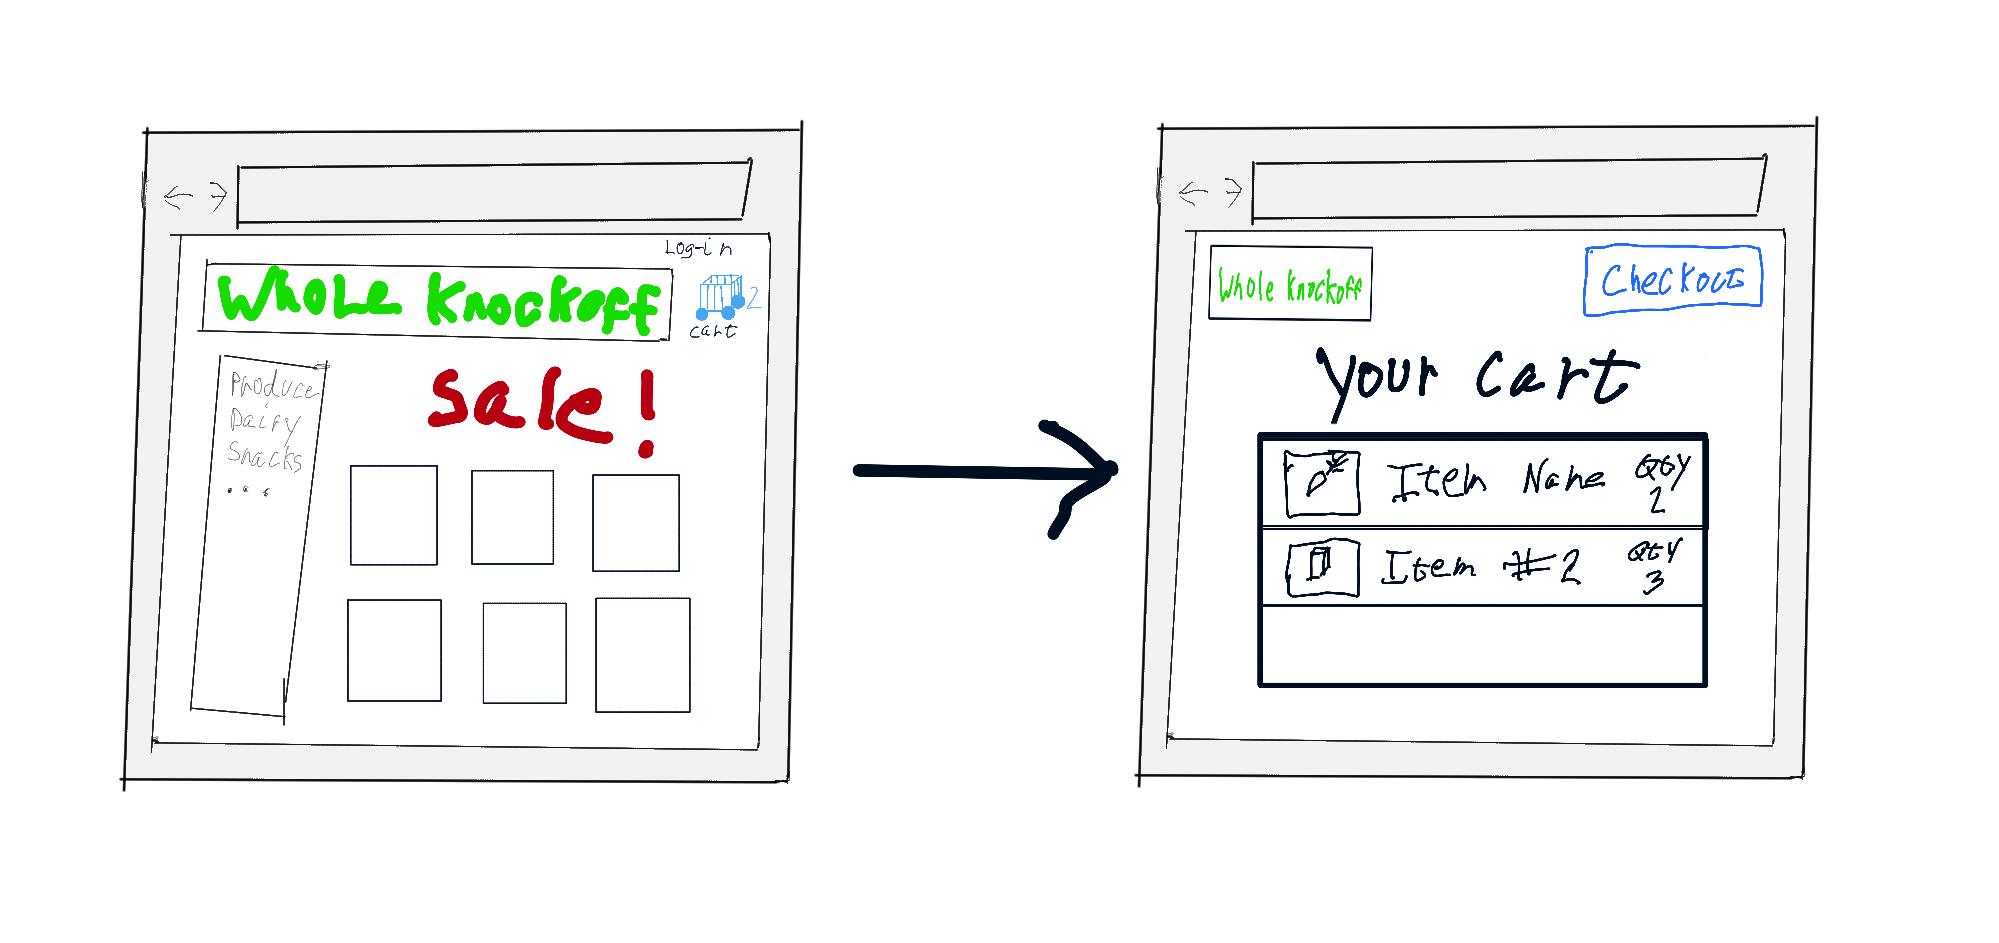
\includegraphics[width=6 in]{1.png}
	%\caption{}
	%\end{figure}
	User Log-in:\\
	%\begin{figure}[p]
	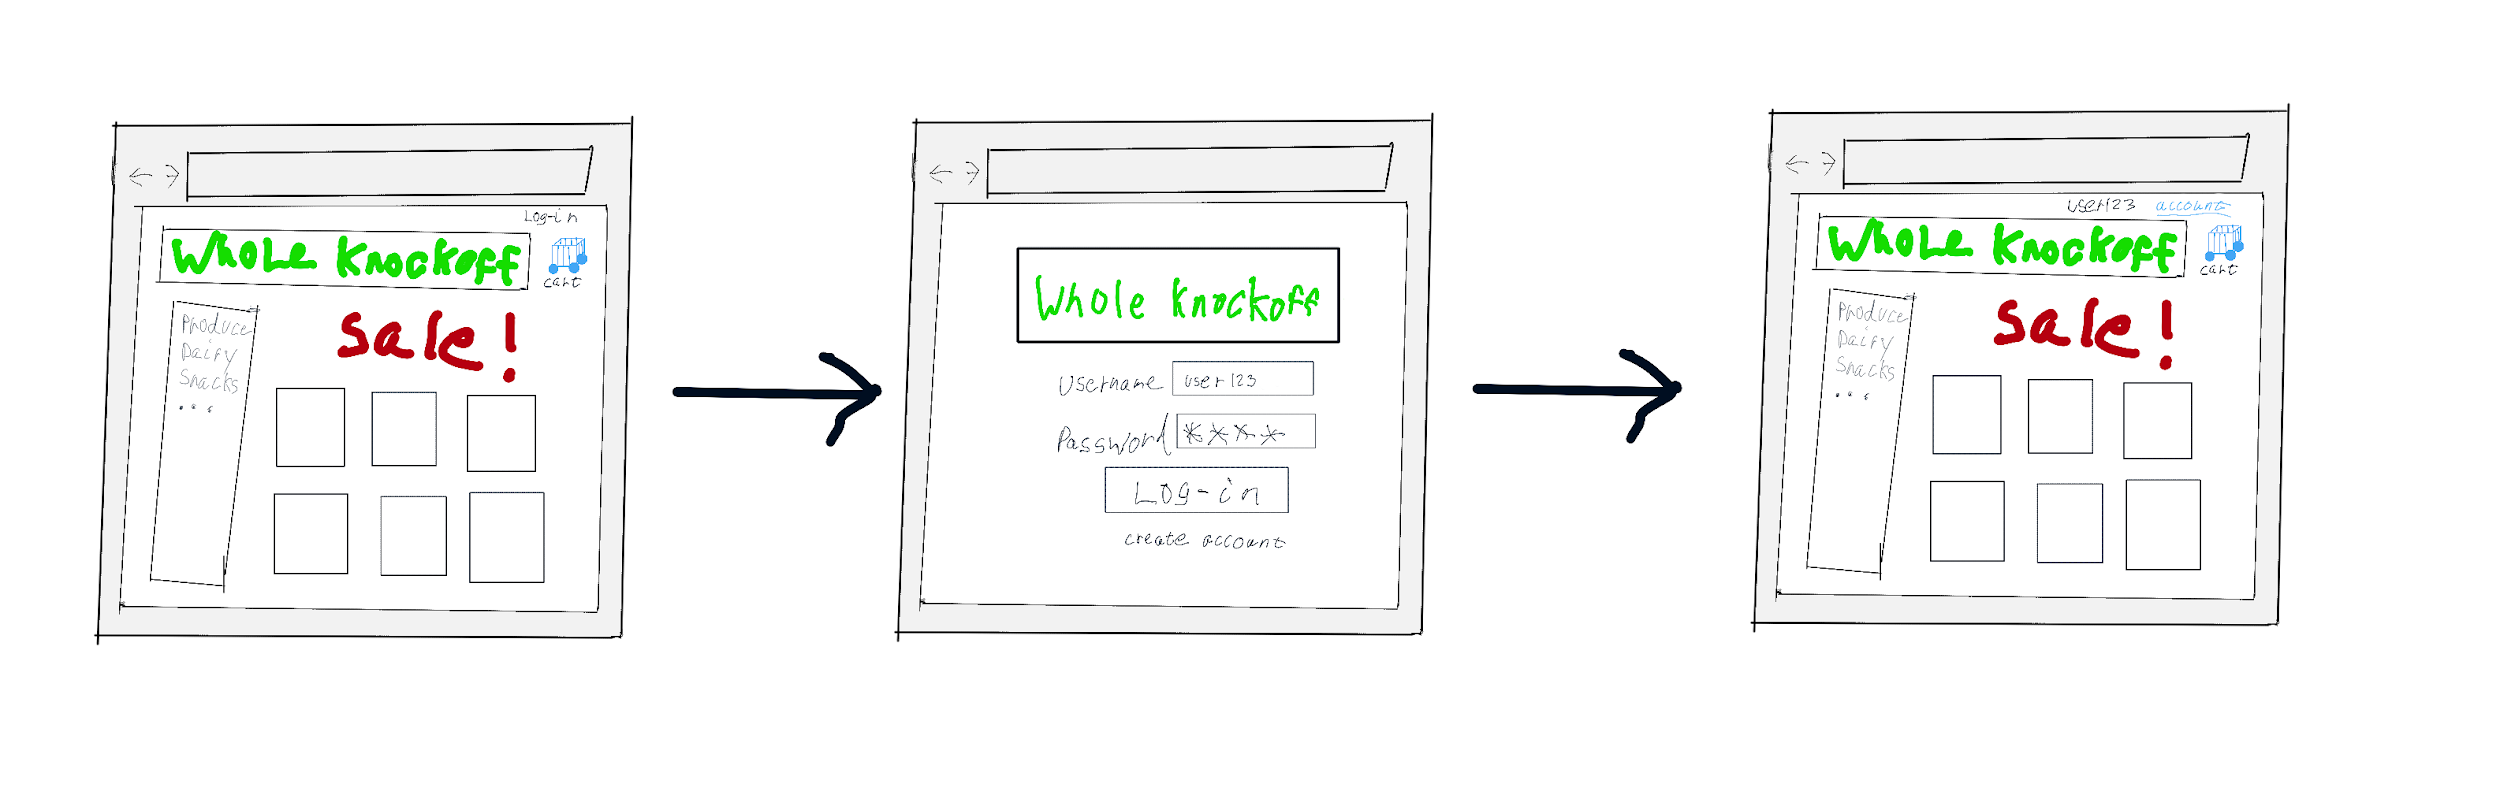
\includegraphics[width=6 in]{2.png}
	%\caption{}
	%\end{figure}
	Employee Order Queue:\\
	%\begin{figure}[p]
	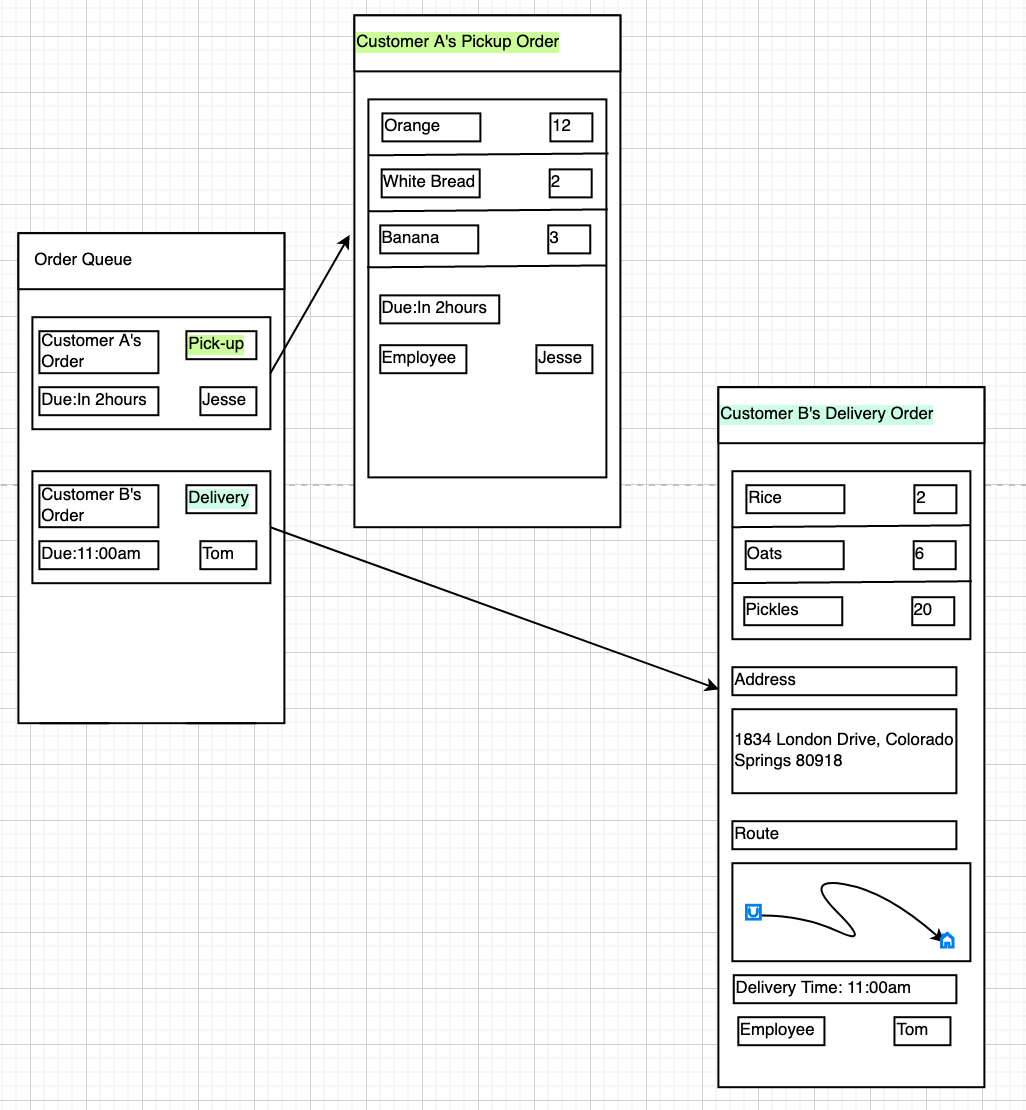
\includegraphics[width=6 in]{3.png}
	%\caption{}
	%\end{figure}
	Options to add item into cart or shopping list:\\
	%\begin{figure}[p]
	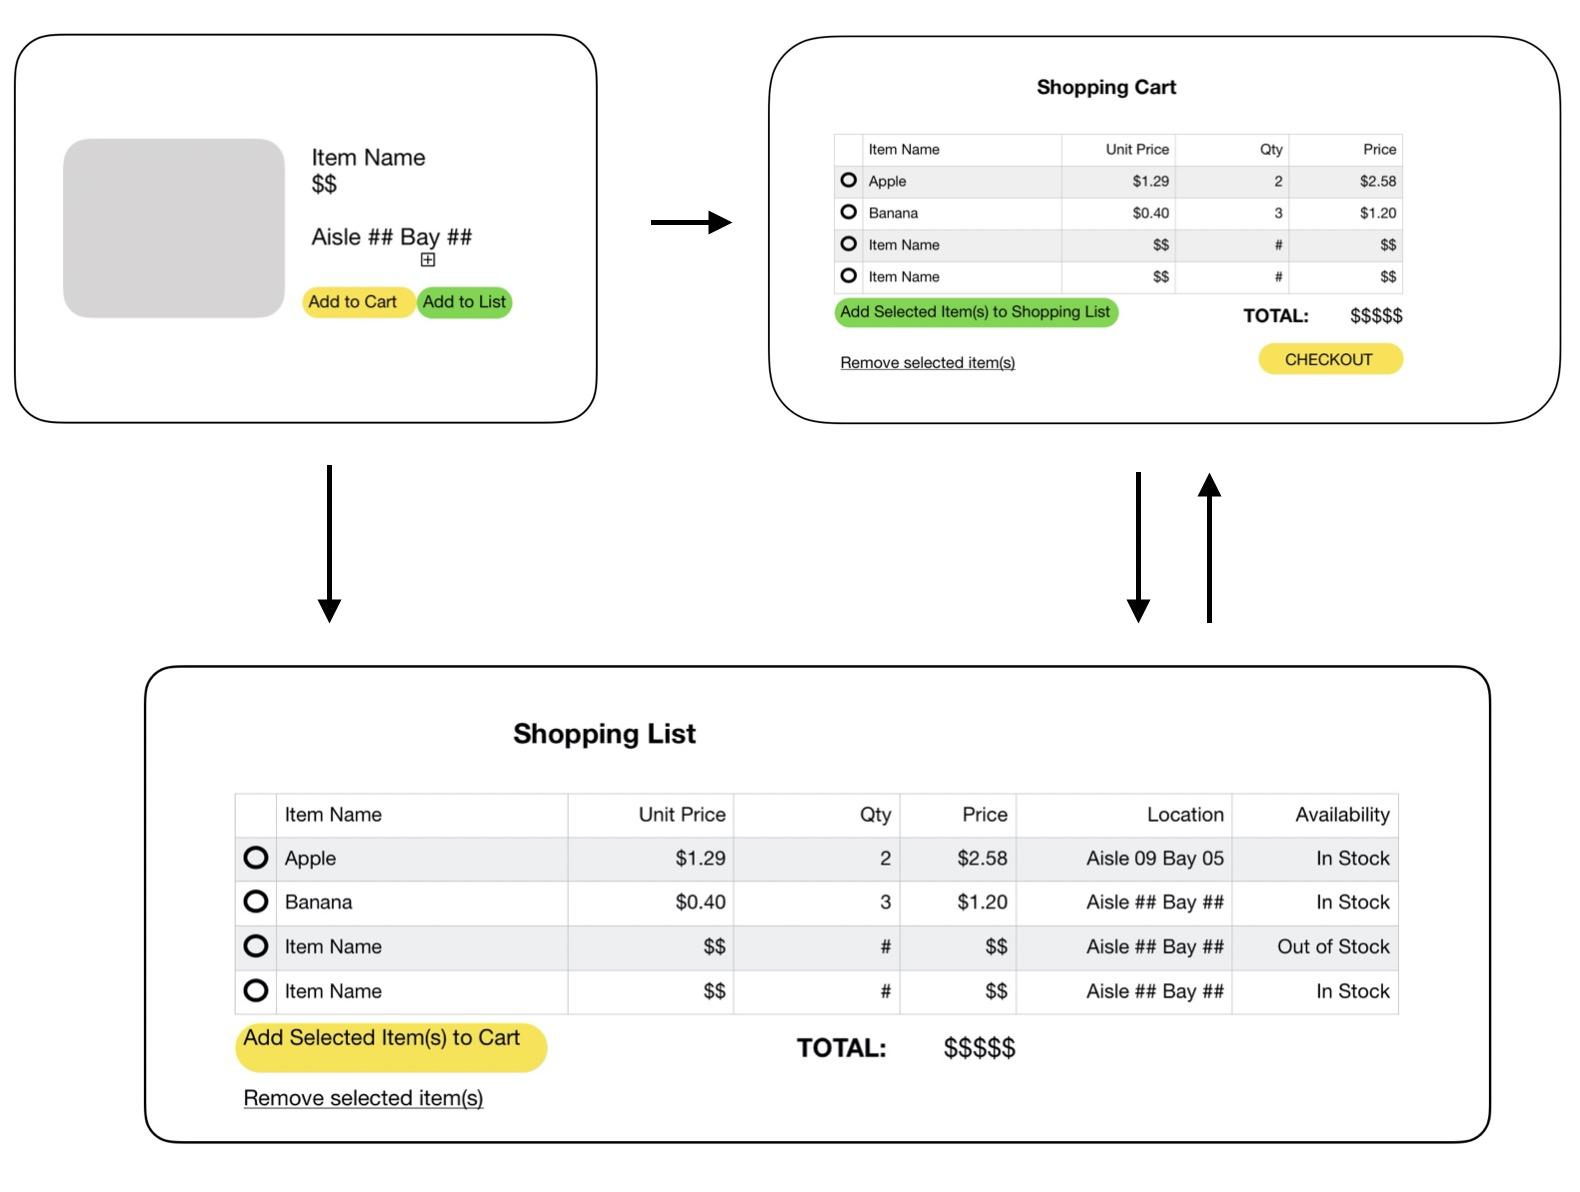
\includegraphics[width=6 in]{4.jpg}
	%\caption{}
	%\end{figure}
	
	\section{Appendix C: }%To Be Determined List}
	$<$ Placeholder $>$
	
\end{document}